\scanpage{62}
\mspage{\textcircled{2}}
% printed form
% @ top, printed form, left column, lines 1–2 | text
MINISTERE DE L'EDUCATION NATIONALE\\
ACADEMIE D'AIX-MARSEILLE\\
\rule{1cm}{0.3pt}

% @ top, printed form, left column, lines 3–4 | text
Inspection Académique\\
de Vaucluse\\
\rule{1cm}{0.3pt}

% @ top, printed form, left column, lines 5–6 | text
Tél. : 90 82 99 76\\
Référence : Secrétariat n\textsuperscript{o}

% @ top, printed form, right column, line 1 | letter part
AVIGNON, le

% @ top, printed form, right column, lines 2–5 | letter part
L'Inspecteur d'académie,\\
directeur des services départementaux\\
de l'Education Nationale de Vaucluse,\\
à M


% @ upper third, below letterhead | diagram
\diagram{\handwritten{\begin{tikzcd}[ampersand replacement=\&]
 x\arrow[r,bend left=19]\arrow[r] \& a
\end{tikzcd}}}

% @ upper middle, line beneath arrows | display
\[
 \handwritten{\pi_0(S_{/x})\unsure{=|\rightrightarrows}\pi_0(S_{/a})}
\]

% @ middle left, two crossing regions | drawing
\figure{\handwritten{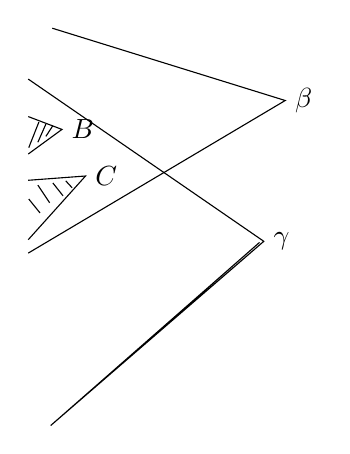
\begin{tikzpicture}[x=.68cm,y=.68cm]
\draw (.45,5.8)--(4.8,4.45)--(0,1.6);
\draw (0,4.85)--(4.4,1.82)--(.42,-1.62)--(4.32,1.8);
\node[right] at (4.8,4.45) {$\beta$}; \node[right] at (4.4,1.82) {$\gamma$};
\draw (0,4.15)--(.63,3.91)--(0,3.45);
\draw (.20,4.05)--(.01,3.57) (.33,4.01)--(.18,3.67) (.46,3.98)--(.33,3.78);
\node[right] at (.63,3.91) {$B$};
\draw (0,2.96)--(1.07,3.04)--(0,1.85);
\draw (.01,2.61)--(.22,2.35) (.18,2.87)--(.40,2.54) (.46,2.91)--(.65,2.67) (.7,2.95)--(.82,2.82);
\node[right] at (1.07,3.04) {$C$};
\end{tikzpicture}}}

% @ middle centre, two tiers of strokes | diagram
\diagram{\handwritten{\begin{tikzcd}[ampersand replacement=\&,row sep=tiny,column sep=tiny]
 \& {}\\
 {}\arrow[ur]\arrow[r] \& {}\\
 {}\arrow[ur,no head]\arrow[r,no head] \& \circ\arrow[d,no head]\\
 \deleted{\unsure{a}}\arrow[r] \& b\arrow[dr,no head]\\
 \phantom{x}\arrow[rr] \& \& x
\end{tikzcd}}}

% @ middle right, line above the vertical pair | display
\[
 \handwritten{\pi_0(\unsure{\mathcal E|\varepsilon|E}_{/x})\simeq}
\]

% @ middle right, vertical pair | diagram
\diagram{\handwritten{\begin{tikzcd}[ampersand replacement=\&]
 \operatorname{Hom}(a,x)\times\mathcal E\arrow[d,shift right]\arrow[d,shift left,no head]\\
 \operatorname{Hom}(a,a)\times\mathcal E
\end{tikzcd}}}

% @ lower third, heading and lines 1–7 | text
\handwritten{\uline{Lemme} Soit $X$ \deleted{dans} Cat \deleted{\unsure{catégorie ayant}} avec quatre objets $B,\ C,\ \beta,\ \gamma$ telle que $\operatorname{Hom}(B,\beta)$, $\operatorname{Hom}(B,\gamma)$, $\operatorname{Hom}(C,\beta)$, $\operatorname{Hom}(C,\gamma)$ \unsure{sont|soient} $\ne\varnothing$, que $B\times C\unsure{=|\ne}\varnothing_{X^\wedge}$ i.e $\nexists x$ \inserted{$\in\operatorname{Ob}X$} avec $\operatorname{Hom}(x,B)\ne\varnothing$ et $\operatorname{Hom}(x,\unsure{e|C})\ne\varnothing$, et $\beta\amalg\gamma=\varnothing_{X^\vee}$ i.e. n'existe pas de $y\in\operatorname{ob}X^\circ$ avec $\operatorname{Hom}(\beta,y)\ne\varnothing$, $\operatorname{Hom}(\gamma,y)\ne\varnothing$. (hyp auto duales). Alors $X$ n'est pas $1$-connexe.}
% slanted
\margin{\handwritten{faux, il faut au moins \deleted{\unsure{supp}} supposer \unsure{en un|en un obj} $x$ tel que $\operatorname{Hom}(x,\beta\times\gamma)\ne\varnothing$, \unsure{on a} $\operatorname{Hom}(x,B)\ne\varnothing$ ou $\operatorname{Hom}(x,C)\ne\varnothing$}}

% @ bottom left, four objects and intervening point | diagram
\diagram{\handwritten{\begin{tikzcd}[ampersand replacement=\&,column sep=small,row sep=tiny]
 B\arrow[dr] \& \& \beta\\
 \& \circ\arrow[ur]\arrow[dr] \& \\
 C\arrow[ur] \& \& \gamma
\end{tikzcd}}}
% archive sheet number: 61
